%==============================================================================%
%================================== intro =====================================%
\section{Introduction}
\subsection{LBGB au sein du Genoscope et du CEA}
Le Genoscope (CNS\footnote{Centre National de Séquençage}) a été créé en 1996 pour participer au projet mondial de séquençage du génome humain (\emph{Human Genome Project}) qui à débuté en 1988 et c'est terminé en 2007, notament dans l'objectif de séquencer le chromosomes 14 humain. Lors de sa cration le Genoscope à égalment été missioné de développer des programmes de génomiques en france dans le cadre du projet France génomique.  Aujourd'hui un des projet phare du Genoscope est le projet \textbf{Tara Océans}, qui  a pour objectifs l'étude des écosystèmes marins planctoniques.

\begin{minipage}{0.40\textwidth}
\begin{figure}[H]
    \centering
    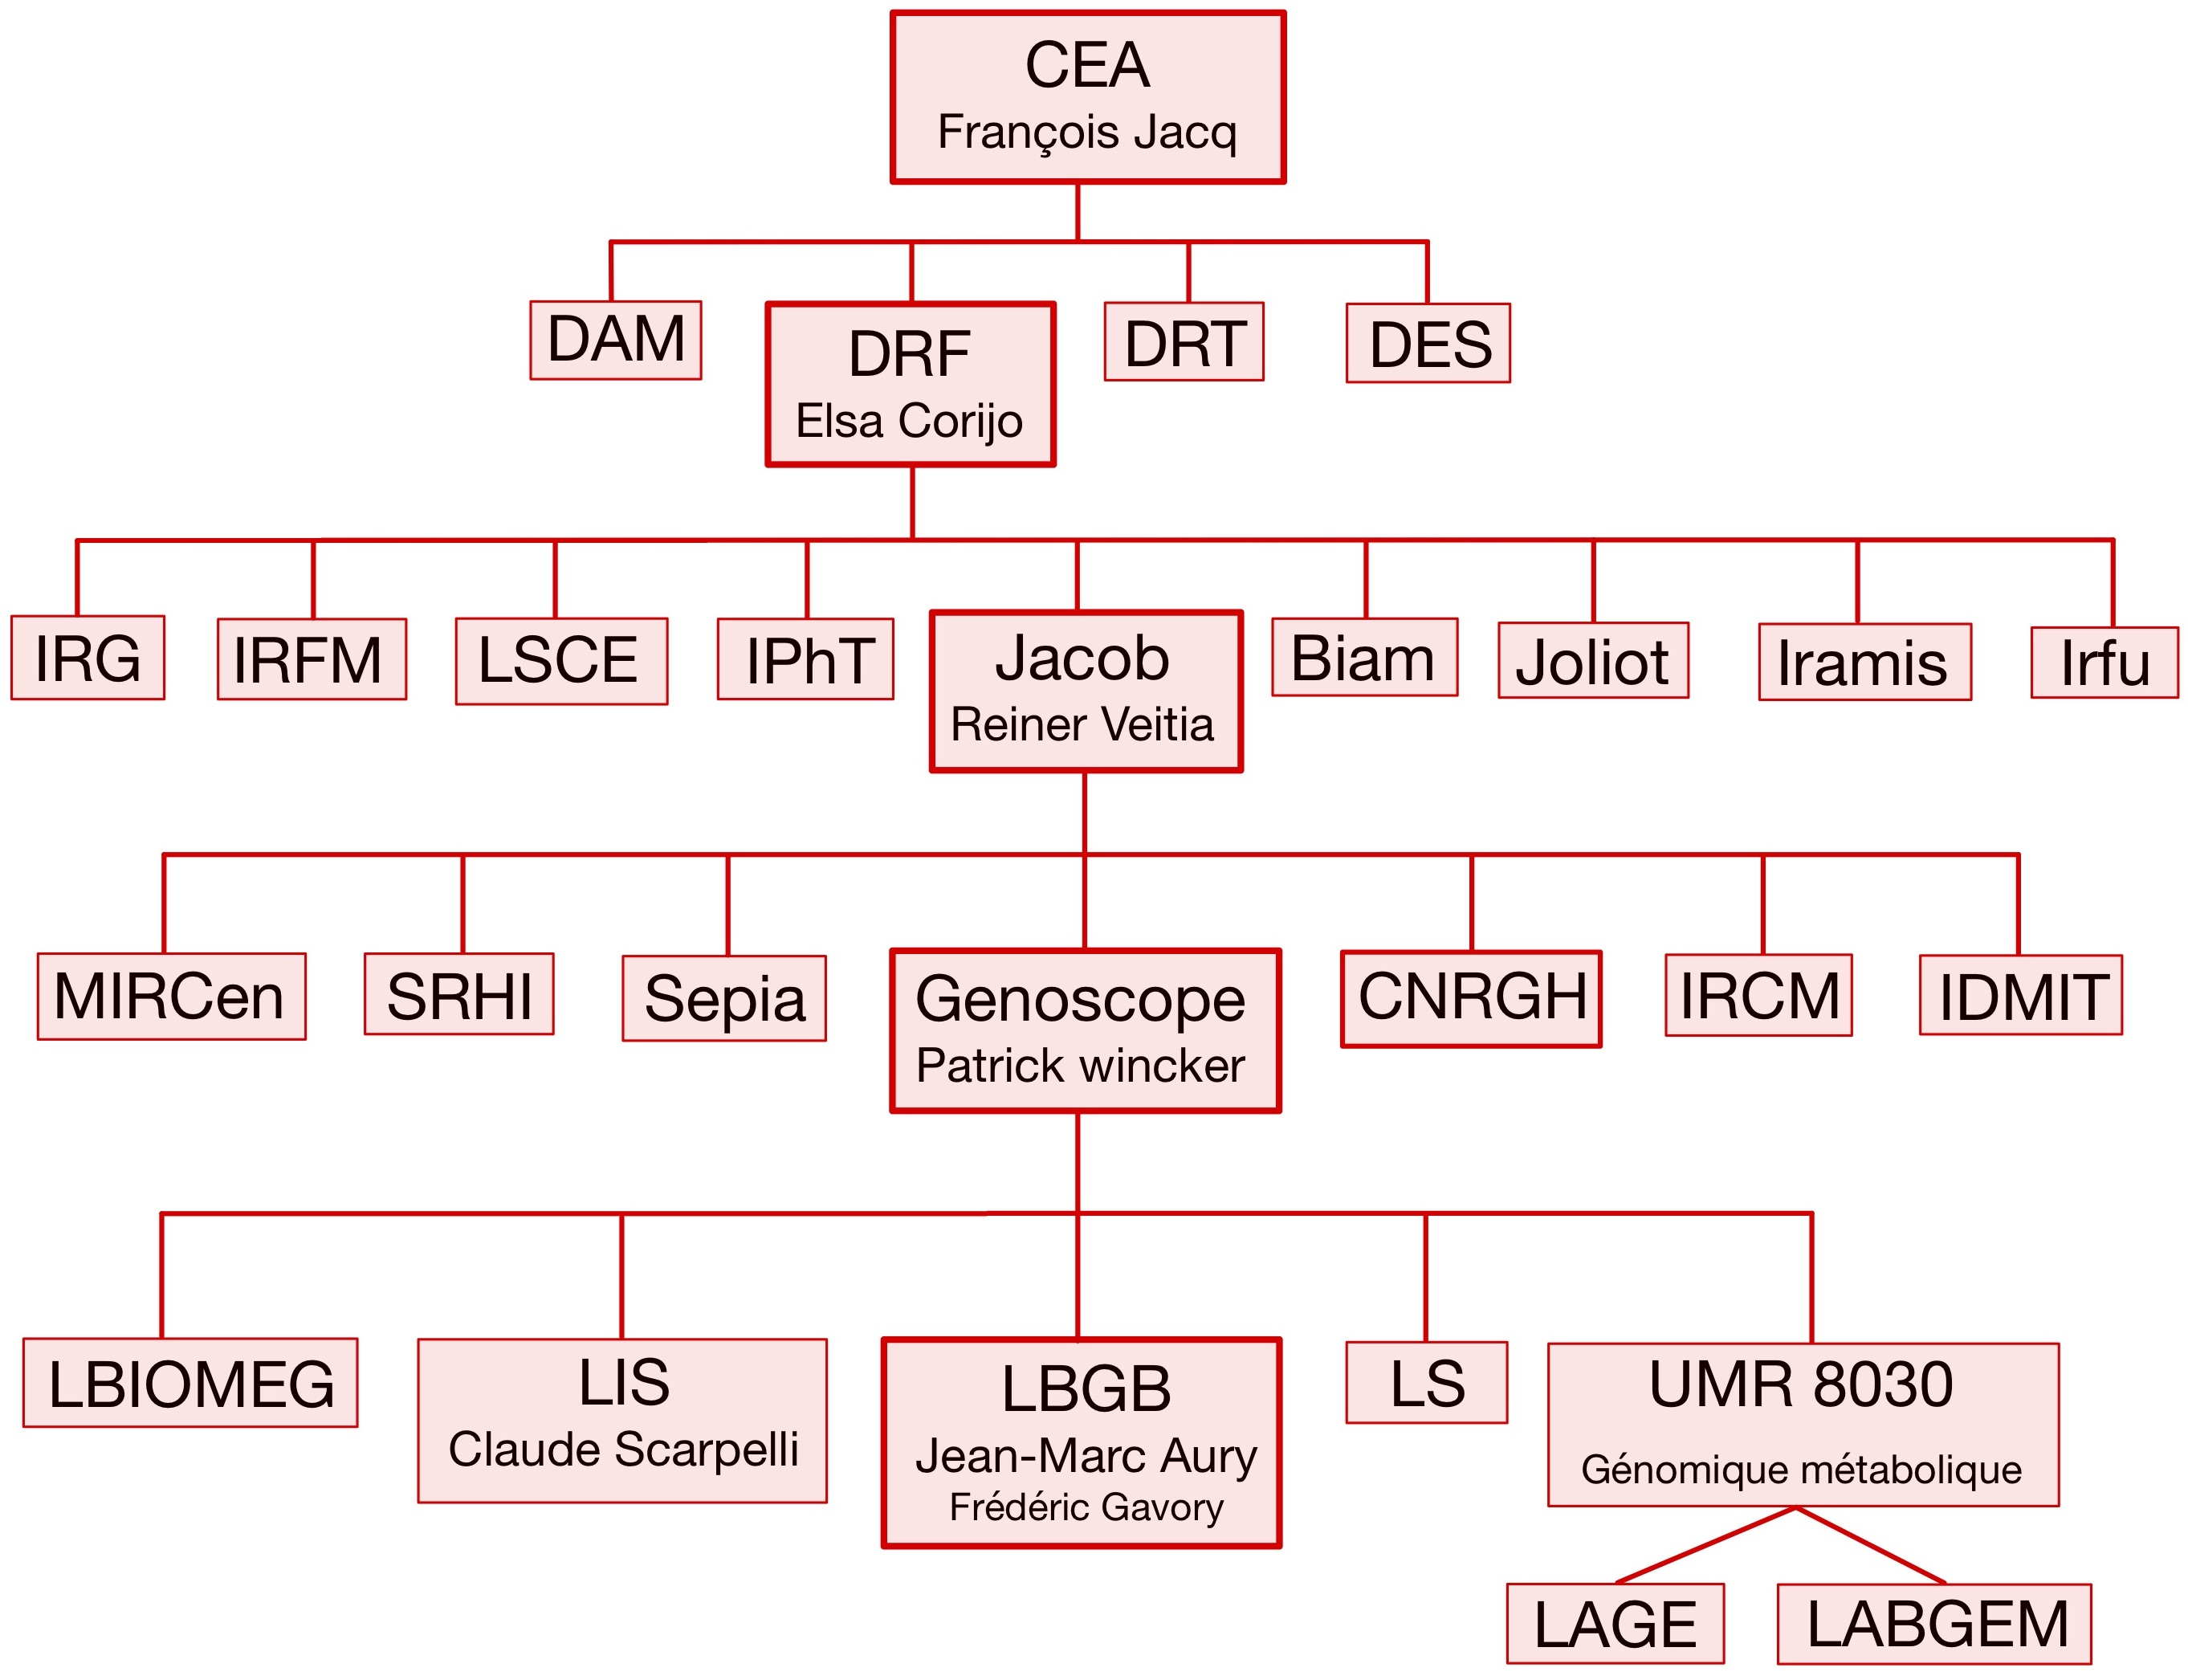
\includegraphics[width=1\textwidth]{img/organigramme.jpg}
    \caption{Organigramme situant l’équipe du Laboratoire de Bioinformatique pour la Génomique et la Biodiversité (LBGB) au sein du Genoscope et du CEA}
    \label{organigramme_LBGB}
\end{figure}
\end{minipage} 
\hfill
\begin{minipage}{0.5\textwidth}
    Le laboratoire de bioinformatique pour la génomique et la biodiversité (\textbf{LBGB}) dirigé par Jean-Marc Aury, fait partie du Genoscope qui est une direction de l'institut François Jacob (Jacob) de la direction de la recherche fondamental (\textbf{DRF}) du Commissariat à l'énergie atomique et aux énergies (\textbf{CEA}), comme on peut l'observé sur l'organigramme de la figure \ref{organigramme_LBGB} qui situe la laboratoire au sein du Genoscope et de CEA. L'intégration du génoscope au CEA à été réaliser en 2007 et en 2017 il dvient une direction de l'institut François Jacob.
\end{minipage}

\subsection{Contexte et missions du LBGB}
Les missions qui sont confié au LBGB est de réaliser de la vielle technologique, de réaliser le contrôle qualité des fichiers de séquences issue des différents séquenceurs. Il à également la missions de réaliser l'assemblage et l'annotation des séquences et des génomes, tout en faisant de la visualisation pour chacune de ces missions. Le Laboratoire est divisé en plusieurs groupes de travails. Le groupe production (dont je fais parti), le groupe assemblage, le groupe d'annotation et le groupe d'évaluation des technologies de séquençage. Les misssions du groupe de production sont de réaliser de la vielle technologique, d'évaluer de nouveux outils, de développer, tester et maintenir les scripts dans l'objectif de répondre aux besoins des équipes de recherche et de séquençage. Notament dans la mise en place et au maintient de pipelines automatiques pour la génération des fichiers de séquences, le contrôle qualité et les analyses biologiques de ces derniers.
%==============================================================================%
%=============================== Objectifs ====================================%
\section{Ojectifs}
Les objectifs de ma mission est la mise en place d'un workflow pour les séquenceurs de la marque \textsc{MGI} dû à l'aquisition de 2 DNBSEQ-G400 et 1 DNBSEQ-T7 par le Genoscope.

\begin{figure}[H]
	\centering
	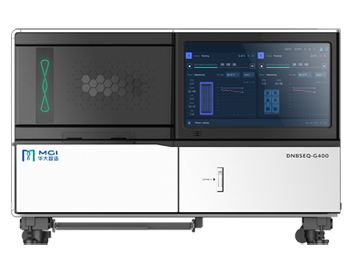
\includegraphics[width=0.3\textwidth]{img/MGI_G400.jpg}
    \hspace{2.5cm}
    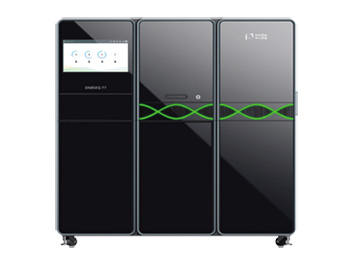
\includegraphics[width=0.3\textwidth]{img/MGI_T7.jpg}
    \caption{Sequenceurs DNBSEQ-G400 (à gauche) et DNBSEQ-T7 (à droite) de \textsc{MGI} \href{https://en.mgi-tech.com/products/}{https://en.mgi-tech.com/products/}}
	\label{seq-MGI}
\end{figure}

Il s'agit de séquenceurs à haut débit équavalent à un HiSeq 4000 pour le DNBSEQ-G400 et à un NovaSeq 6000 pour le DNBSEQ-T7 de chez \textsc{Illumina}. L'objectif sera de créer un worflow de pipelines similaire à celui présenté ci-dessous.

\begin{minipage}{0.45\textwidth}
	\begin{figure}[H]
		\centering
		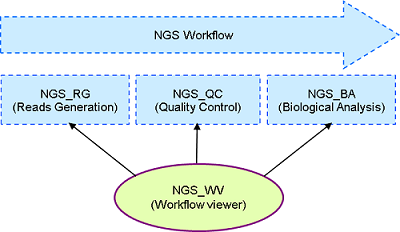
\includegraphics[width=1\textwidth]{img/Workflow.png}
		\caption{Workflow de génération, de controle qualité et d’analyse biologique des FASTQ}
		\label{worflow-genoscope}
	\end{figure}
\end{minipage} 
\hfill
\begin{minipage}{0.45\textwidth}
	Plus précissément il s'agira de créer un pipelines de génération de reads (\textsc{NGS\_RG-MGI}) et un pour le contrôle qualité (\textsc{NGS\_QC-MGI}). C'est deux étapes sont la condition pour que les fichiers de séquences brut soit tranféré sur bande magnétique et effacé de la base de données de références (\textsc{NGL}). 
\end{minipage}\\

Ces pipelines ont pour tâches de réaliser la distribution des fichiers \textsc{FASTQ} par projet, de les trier par échantillons, runs et technologies. Ainsi que de réaliser le nettoyage et l'analyse des fichiers \textsc{FASTQ}, tout en  mettant à jour la base de données \textsc{NGL}.\\

Les autres objetifs de ma mission est de réaliser des évaluations d'outils utilisé et de nouveaux outils pour les différents pipelines en place pour les différentes technologies de séquençage. Tel que l'évaluation d'outils de génération de fichier \textsc{FASTQ} et de démultiplexage, des outils de \emph{flitering}, \emph{trimming}, ect. Ainsi que de maintenir les pipelines des différentes technologies en ajoutant, remplaçant, ou stopant certains outils suite à une évaluation de ces derniers ; notament pour le workflow d'\textsc{Illumina} et celui de \textsc{MGI} une fois ce dernier créé.
%==============================================================================%
%================================ Méthodes ====================================%
\section{Matériels et Méthodes}
L'écriture du workflow de pipelines pour les séquenceurs \textsc{MGI} sera réaliser dans le langage de programmation \textsc{Perl}. L'utilisation de ce langage est fait pour des raison historique du laboratoire, puisque de nombreuses librairies et modules qui seront à utiliser dans l'écriture des pipelines sont écrit en \textsc{Perl}. le workflow pour \textsc{MGI} s'appuirera sur le workflow d'\textsc{Illumina} qui est totalement implémenté en \textsc{Perl}. C'est pour toutes ses raisons qu'il m'a été nécessaire d'apprendre à coder en \textsc{Perl}. \\

Une première évaluation d'outils à également été efféctué. Il s'agit de comparer les performance de deux logiciels de génération de fichiers \textsc{FASTQ} ainsi que leurs démultiplexage. Il s'agit donc de comparer les performance entre le logiciel utilisé actuelment au Genoscope, qui est \textsc{bcl2fastq}, avec le logiciel \textsc{bcl-convert} qui sont tous deux developper et commercialisé par \textsc{Illumina}.\\
Dans un premier temps il sera necessaire de déterminer la meilleur combinaison de paramètre pour \textsc{bcl2fastq}, pour pouvoir appliquer les mêmes paramètres pour \textsc{bcl-convert}. Les paramètres en question sont :
\begin{itemize}
    \item[•] \texttt{r} : nombre de \emph{threads} accordé pour la décompréssion et la lecture des \emph{Bases Calls}
    \item[•] \texttt{p} : conversion des \emph{Bases Calls} en \textsc{FASTQ}
    \item[•] \texttt{w} : écriture et compréssion des fichier \textsc{FASTQ}
\end{itemize}
Les paramètres èquivalent pour le logiciel \textsc{bcl-convert} sont 
\begin{itemize}
    \item[•] \texttt{bcl-num-decompression-threads} : nombre de \emph{threads} accordé pour la décompréssion et la lecture des \emph{Bases Calls}
    \item[•] \texttt{bcl-num-conversion-threads} : conversion des \emph{Bases Calls} en \textsc{FASTQ}
    \item[•] \texttt{bcl-num-compression-threads} : écriture et compréssion des fichier \textsc{FASTQ}\\
\end{itemize}

Tous ces tests ont été  réalisés sur le même noeud de calcul, dans l'objectif de minimiser les biais que pourrait produire de faire une comparaison sur des resultats provenant de noeud de calcul différent. LA comparaison est effactué sur le temps total pour la génération des \textsc{FASTQ} et le démultiplexage, ainsi que le temps cpu et le pourcentage d'utilisation des cpu.

%==============================================================================%
%================================ Resultats ===================================%
\section{1$^{\text{er}}$ Résultats}
Suite à l'apprentissage du \textsc{Perl} en réalisant un programme permettant de faire des analyses statistiques élémentaire sur des fichiers \textsc{FASTQ}. Tel que le taux de GC, la moyenne du score de la qualité, ainsi que plusieurs autres métriques. Le programme est capable de gérer les fichiers \textsc{FASTQ} issue de séquençage \emph{single end} et \emph{paired end}. Cela m'a permis de prendre en main les modules utilisé pour les différents pipelines déja en place, notament pour  le pipelines d'\textsc{Illumina}. À la suite de cette prise en main de l'environement de travail, l'utilisation du lancement de job sur les noeuds de calculs, l'apprentissage du \textsc{Perl} et l'utilisation des modules utilisé pour le workflow d'\textsc{Illumina}. On a réaliser une comparaison entre deux logiciels de génération de \textsc{FASTQ} et de démultiplexage.

\subsection{Détermination des meilleurs paramètres pour \textsc{bcl2fastq}}
Après avoir effectué différentes combinaisons des paramètres, nous avons mis en évidence que la variation du paramètre \texttt{r} et \texttt{w} en fixant le paramètre \texttt{p}, n'apportait pas de différences significatives. Nous avons donc fait varier les paramètres \texttt{p}, \texttt{r} et \texttt{w} de manière à ce que chacun des paramètre soit égale au nombre de coeurs accordé aux deux logiciels.

\subsection{Comparaison entre \textsc{bcl2fastq} et \textsc{bcl-convert}}

\begin{figure}[H]
    \centering
    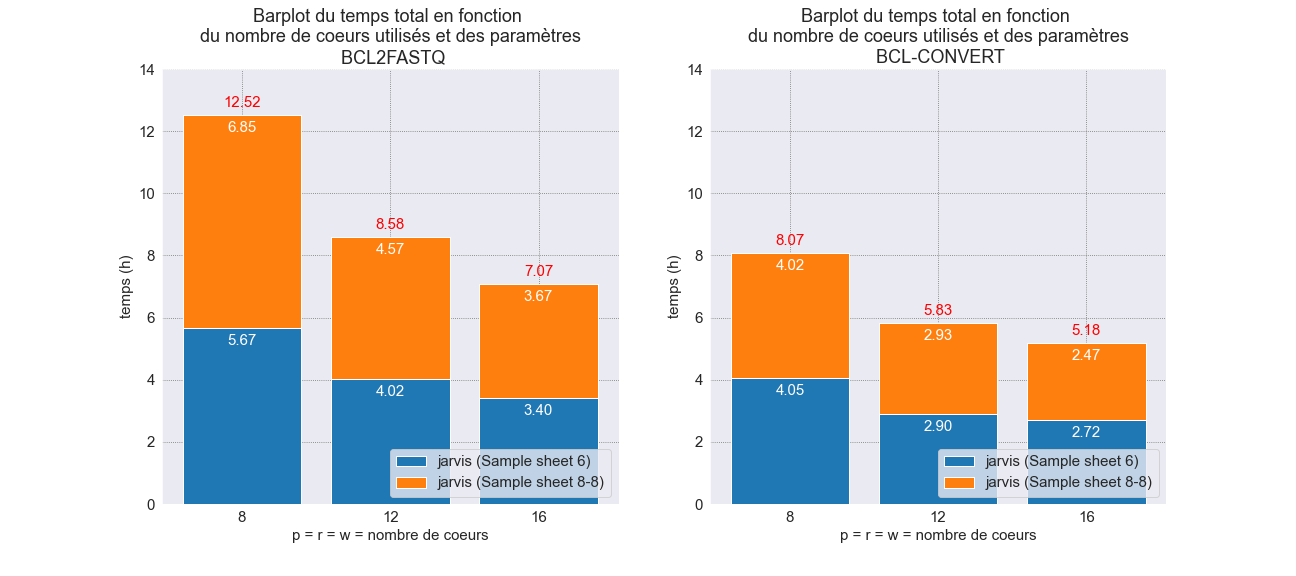
\includegraphics[width=1\textwidth]{img/barplot_total_time_comp.png}
    \caption{Temps total de génération des FASTQ pour bcl2fastq et bcl-convert}
    \label{fig-total-time}
\end{figure} 

La figure \ref{fig-total-time}, montre la différence de temps total des deux logiciels. Il y a deux \emph{sample sheet}, car le nombre de bases considérés des \emph{reads index} entre les \emph{lanes} est différents, obligeant à réaliser deux appelle différents au logiciels pour générer les \textsc{FASTQ} et le démultiplexage. 
On oserve bien que plus on augmente le nombre de coeurs pour chacun des logiciels plus la génération des \textsc{FASTQ} et le démultiplexage est rapide. De plus on remarque que \textsc{bcl-convert} permet de réduire le temps d'environs 1/3 par rapport à \textsc{bcl2fatq}.\\

Il existe un autre paramètre pour \textsc{bcl-convert} qui permet de spécifier le nombre de têche à effectuer en parralèles qui n'existe pas pour \textsc{bcl2fatq}. Il reste donc à détermier si en utilisant ce paramètre et en le faisant varier, cela permetterait de réduire le temps de génération des \textsc{FASTQ} et le démultiplexage. 
%==============================================================================%
%======================== Conclusion et perspectives ==========================%
\section{Perspectives}
Concernant les perspective issue de cette comparaison de logiciels, il reste à déterminer les sorties que textsc{bcl-convert} qui sont différentes de \textsc{bcl2fatq} et de réaliser une adaptation du workflow d'\textsc{Illumina} en concéquence. \\

Concernant le workflow de \textsc{MGI}, il nous faut dans un premier temps déterminer les outils et méthodes necessaires. Notament, déterminer quels sont les outils et méthodes que l'on ré-utilisera du workflow \textsc{Illumina}, des nouveaux outils et méthodes à utiliser ou à développer. Une fois ceci déterminer il restera à écrire les deux pipeline, celui de génération de reads (\textsc{NGS\_RG-MGI}) et celui de contrôle qualité (\textsc{NGS\_QC-MGI}). L'objectif sur le long terme est d'arriver à un workflow totalment automatisé, comme celui \textsc{Illumina}.\\

Il y a aussi l'évaluation d'autres outils utiles pour les pipelines, comme l'évaluation d'outils de \emph{trimming}, \emph{filtering}, d'assignation taxonomique, ect.
\subsection{diagramme de gantt}
